\section{Outras Funções Trigonométricas}
\begin{frame}
\frametitle{Definições} 

\begin{definicao}\label{outrasfunctrig}
Definem-se, através das funções seno e cosseno, as funções
trigonométricas com as seguintes leis de formação:
\begin{itemize}
	\item $\tan x = \frac {\sen x}{\cos x}$, \sub{tangente};
	\item $\cot x = \frac {\cos x}{\sen x}$, \sub{cotangente};
	\item $\sec x = \frac {1}{\cos x}$, \sub{secante};
	\item $\csc x = \frac {1}{\sen x}$, \sub{cossecante}.
\end{itemize}
Os domínios dessas funções não contêm o conjunto dos valores de $x$
que zeram seus respectivos denominadores.
\end{definicao}
Por exemplo, o maior subconjunto dos reais no qual podemos definir
as funções tangente e secante é $$\bigcup_{k \in \Z} \paren{k \pi -
\frac {\pi} 2, k \pi + \frac {\pi} 2}.$$
\end{frame}
%------------------------------------------------------------------------------------------------------------

\begin{frame}
\frametitle{Gráfico da Função Tangente} 

\begin{exemplo}
O gráfico da função $\tan: \bigcup_{k \in \Z} \paren{k \pi - \frac
{\pi} 2, k \pi + \frac {\pi} 2} \to \R$ é:
\begin{center}
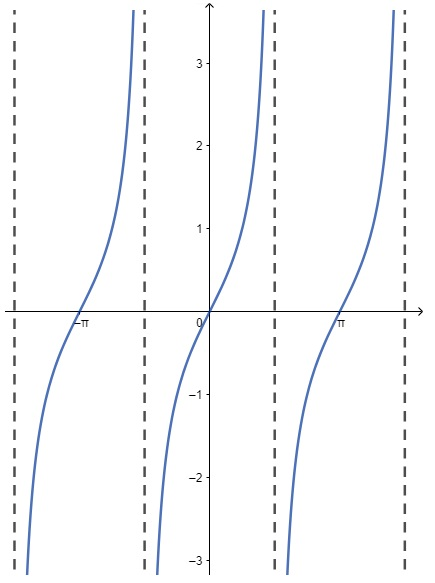
\includegraphics[width=4.6cm]{figures/graftan.jpg}
\end{center}
\end{exemplo}

\end{frame}

%------------------------------------------------------------------------------------------------------------

\begin{frame}
\frametitle{Propriedades da Função Tangente} 

\begin{proposicao}
Valem as seguintes propriedades acerca da função tangente:
\begin{itemize}
	\item Embora não seja definida para todo número real, a função
	tangente pode ser considerada uma função periódica de período
	$\pi$ em todo o seu domínio, pois $\tan \paren{x+\pi} = \tan x$;
	\item Para todo par de pontos  $(x_1, y_1)$ e $(x_2, y_2)$ em uma reta não vertical, com $x_1 \neq x_2$, se
	$\alpha$ é o ângulo formado pela reta e o eixo $x$, então $$\tan
	\alpha = \frac {y_2 - y_1} {x_2 - x_1}.$$
	\item Ao definirmos $tan: \paren{- \frac {\pi} 2, \frac {\pi} 2} \to \R$,
obtemos uma bijeção. Assim, o intervalo aberto $\paren{- \frac {\pi}
2, \frac {\pi} 2}$ tem a mesma cardinalidade que $\R$.

\end{itemize}
\end{proposicao}


\end{frame}

%------------------------------------------------------------------------------------------------------------

\begin{frame}
\frametitle{A Função Inversa da Tangente}  


\begin{exemplo}
Como $tan: \paren{- \frac {\pi} 2, \frac {\pi} 2} \to \R$ é
bijetiva, então essa função possui inversa, que chamamos de
\sub{arco tangente} e denotamos por $\arctan : \R \to
\paren{- \frac {\pi} 2, \frac {\pi} 2}$. Seu gráfico é
\begin{center}
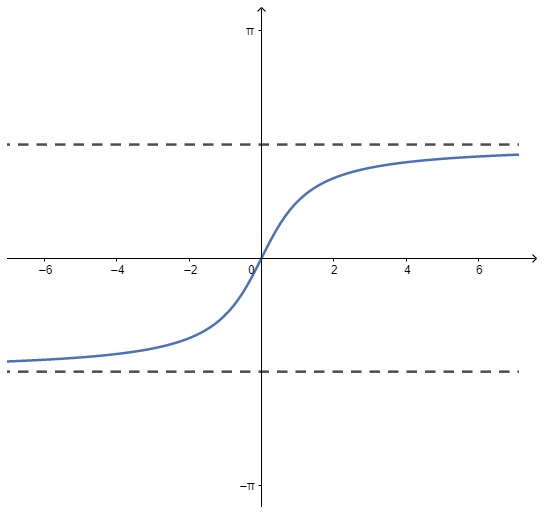
\includegraphics[width=5.5cm]{figures/grafarctan.jpg}
\end{center}
\end{exemplo}


\end{frame}

%------------------------------------------------------------------------------------------------------------